\documentclass{standalone}
%\pagenumbering{gobble}


%%%%%%%%%%%%%%%%%%%%%%%%%%%%%%%%%%%%%%%%%%%%
% HI 21cm line schematic
%
%%%%%%%%%%%%%%%%%%%%%%%%%%%%%%%%%%%%%%%%%%%%


\usepackage{tikz,xcolor}
\usetikzlibrary{arrows, shadings, calc}

%[draw options] (center) (initial angle:final angle:radius)
\def\centerarc[#1](#2)(#3:#4:#5) {\draw[#1] ($(#2)+({#5*cos(#3)},{#5*sin(#3)})$) arc (#3:#4:#5);}

\begin{document}

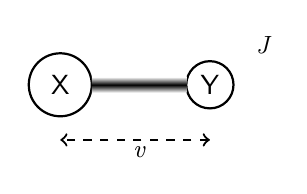
\begin{tikzpicture}[scale=1.0, font=\sffamily]

	% Draw the individual atoms
	\draw[thick] (-1cm,0cm) circle (0.4cm);
	\node[align=center] at (-1,0) {X};
	\draw[thick] (0.9cm,0cm) circle (0.3cm);
	\node[align=center] at (0.9,0) {Y};

	% Draw the bond
	%\draw[style={thick}] (-0.6cm,0cm) -- (0.6cm,0cm);
	%\draw (-0.6,-0.1) rectangle (0.6,0.1);
	\begin{scope}%[transform canvas={rotate=30}]
		\shade[shading=axis,bottom color=white,top color=white,middle color=black,shading angle=0] (-0.6,-0.1) rectangle (0.6,0.1);
	\end{scope}

	% Vibrational motion
	\draw[black, thick, dashed, <->] (0.9cm,-0.7cm) -- (-1cm,-0.7cm);
	\node[align=center] at (0,-0.85) {{\small{\it v}}};
	% add some white space underneath so the arrows are not clipped off the bottom
	%\draw[white] (0cm,-0.8cm) -- (0cm,-0.8cm);

	% Rotational  motion
	\centerarc[black, thick, dotted, ->](0,0)(-25:25:1.5)
	\centerarc[black, thick, dotted, ->](0,0)(158:202:1.7)
	\node[align=center] at (1.57,0.5) {{\small{\it J}}};


\end{tikzpicture}

\end{document} 
